%%%%%%%%%%%%%%%%%%%%%%%%%%%%%%%%%%%%%%%%%%%%%%%%%%%%%%%%%%%%%%%%%%%%%%%
\chapter{Multiport Fields and Junction Structures}
\label{ch:fields}
%%%%%%%%%%%%%%%%%%%%%%%%%%%%%%%%%%%%%%%%%%%%%%%%%%%%%%%%%%%%%%%%%%%%%%%

Real physical components often couple multiple energy flows simultaneously. A flexible beam deformed by two forces stores energy that depends on \emph{both} displacements simultaneously, not independently. A 3D rigid body has coupled translational and rotational inertia. These multi-port couplings cannot be captured by separate 1-port elements — they require \textbf{multiport fields}. 

Using fields and junction structures, it is possible to study systems with complex multiport components using bond graphs because they combine structural detail, clarity, and ease of visualization. 

\begin{insightbox}[Important Assumption for Fields]
All multiport elements that we are going to study in this chapter are assumed to be (and are going to be studied as) \textbf{ALL INWARDS} in terms of power bond directions. This means power is conventionally positive when flowing into the field from all ports.
\end{insightbox}

\section{C-fields: multiport potential energy storage}

A \textbf{C-field} is the multiport generalization of the 1-port C-element. It is itself a distributed compliance element, representing a distributed hole of energy conservation. It has $n$ ports, and its potential energy is a function of all $n$ displacements simultaneously:
\begin{equation}
  E(\mathbf{q}) = \int_{0}^{t} \sum_{i=1}^{n} e_i f_i d\tau = 
  \int_{0}^{t} \sum_{i=1}^{n} e_i \dot{q}_i d\tau = 
  \int_{0}^{t} \sum_{i=1}^{n} e_i(\mathbf{q}) dq_i =  
  \int_{\mathbf{q}_0}^{\mathbf{q}} \mathbf{e}(\bar{\mathbf{q}})^T\,d\bar{\mathbf{q}}, \qquad
  e_i = \frac{\partial E}{\partial q_i}(\mathbf{q}).
\end{equation}

This means that a change in any component is going to cause a change in the stored energy. Because $E(\mathbf{q})$ represents stored potential energy, the C-field inherently conserves energy.

\begin{insightbox}{Advantage of Fields}
  The advantage of Fields is that they allow us to capture the physics of multiport energy storage directly, without needing to break it down into multiple 1-port elements and junctions. Moreover, a C-field can be thought of as a \textbf{Inertia} \textbf{Compliance} \textbf{Damping} Matrix that captures the coupling between ports in a compact way without the need of explicitly writing the internal structure of the filed. 
\end{insightbox}


The constitutive law is a set of $n$ functions $e_i(\mathbf{q})$ giving the efforts at each port as a function of all displacements. By inspection, $\mathbf{e}(\mathbf{q}) = \nabla E(\mathbf{q})$. For the C-field to be physically meaningful (\textbf{conservative}), the energy function $E(\mathbf{q})$ must exist, which requires the \textbf{Maxwell reciprocal relations} (a structural constraint):
\begin{equation}
  \frac{\partial e_i}{\partial q_j} = \frac{\partial^2 E}{\partial q_i \partial q_j} = \frac{\partial e_j}{\partial q_i} \quad \forall\, i,j.
  \label{eq:maxwell}
\end{equation}
This is the direct multivariable generalization of the single-port condition $e = \partial E/\partial q$. It is clear that not every arbitrary set of constitutive laws expressing efforts in terms of displacements could come from a valid energy-storing C-field—only those sets that obey this symmetry property!

\paragraph{Compliance and stiffness forms.}
If the constitutive law can be written $\mathbf{q} = \mathbf{M}_c(\mathbf{e})$ (displacements as functions of efforts), this is the \textbf{compliance form}. If it can be written $\mathbf{e} = \mathbf{M}_k(\mathbf{q})$ (or $\mathbf{M}_c^{-1}(\mathbf{q})$), this is the \textbf{stiffness form}. 

In the linear case, the equations become:
\begin{equation}
  \mathbf{e} = \mathbf{K}\,\mathbf{q} \quad (\text{stiffness}), \qquad
  \mathbf{q} = \mathbf{C}\,\mathbf{e} \quad (\text{compliance}),
\end{equation}
where $\mathbf{K} = \mathbf{C}^{-1}$ is the stiffness matrix and $\mathbf{C} = \mathbf{M}_c$ is the compliance matrix. The stored energy is $E = \frac{1}{2}\mathbf{q}^T\mathbf{K}\mathbf{q}$. Maxwell reciprocity requires $\mathbf{K} = \mathbf{K}^T$ and $\mathbf{C} = \mathbf{C}^T$ (symmetric matrices), a familiar result from structural mechanics.

\begin{example}[Elastic beam loaded at two points]
An Euler-Bernoulli beam of length $L$, stiffness $EI$, loaded by forces $F_1$ at $L/3$ and $F_2$ at $2L/3$ has the compliance matrix:
\begin{equation}
  \begin{pmatrix}x_1\\x_2\end{pmatrix}
  = \frac{L^3}{243EI}\begin{pmatrix}4&\frac{7}{2}\\\frac{7}{2}&4\end{pmatrix}
  \begin{pmatrix}F_1\\F_2\end{pmatrix}.
\end{equation}
The symmetric compliance matrix confirms Maxwell reciprocity. 
\end{example}


\paragraph{Nonlinear C-fields.}
Nonlinear C-fields are common in certain application areas. A mechanical element that behaves as a linear 1-port in restricted cases can often be modelled as a nonlinear 2-port C-field when two-dimensional motion is permitted. 

\begin{figure} [H]
  \centering
  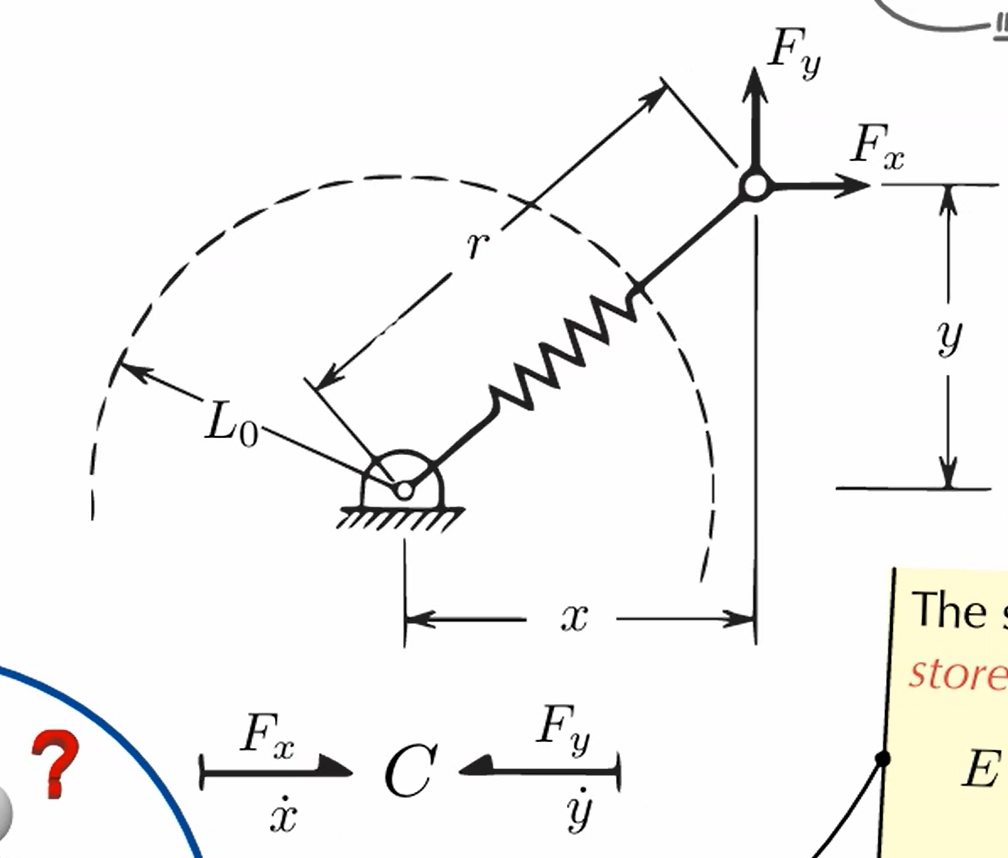
\includegraphics[scale=0.25]{figs/chapter5/5_3.png}
  \caption{A simple linear spring pivoting in a 2D plane is a nonlinear C-field.}
\end{figure}


For example, a simple linear spring (rest length $L_0$, stiffness $k$) pivoting in a 2D plane ($x, y$) has the energy:
\begin{equation}
  E(x,y) = \frac{1}{2}k\left(\sqrt{x^2+y^2} - L_0\right)^2
\end{equation}
The gradient of this potential energy gives the highly nonlinear constitutive equations for the $x$ and $y$ efforts:
\begin{equation}
  F_x = kx - k\frac{L_0 x}{\sqrt{x^2+y^2}}, \qquad F_y = ky - k\frac{L_0 y}{\sqrt{x^2+y^2}}
\end{equation}

\subsection{Explicit vs.\ implicit C-fields}

An \textbf{implicit field} arises when a group of 1-port C-elements, connected by junction structures (0-junctions, 1-junctions, TF), collectively behaves as a C-field. For example, two springs $k_1$ and $k_2$ connected in series via a 1-junction (sharing a common force, but adding displacements) or connected in parallel via a 0-junction form an implicit C-field. The implicit form is naturally obtained from the assembly of the bond graph; converting it to explicit form requires solving for the field's constitutive equations algebraically.

\begin{figure}[H]
  \centering
  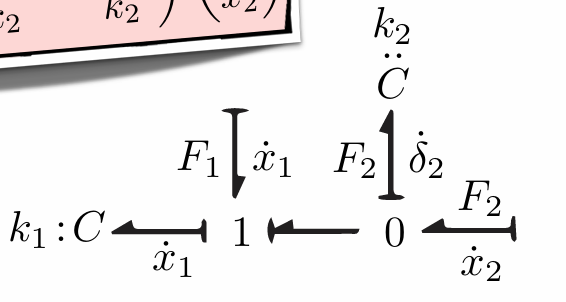
\includegraphics[scale=0.25]{figs/chapter5/5_1.png}
  \caption{Implicit C-field}
\end{figure}

An \textbf{explicit field} is one whose constitutive law is given directly as $\mathbf{e}(\mathbf{q})$ or $\mathbf{q}(\mathbf{e})$ — the multiport is defined from the outset as a single entity (like the beam example above). 

\begin{figure}[H]
  \centering
  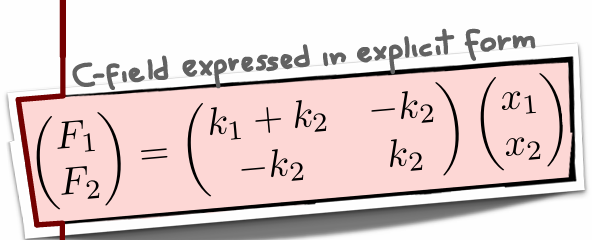
\includegraphics[scale=0.25]{figs/chapter5/5_2.png}
  \caption{Explicit C-field}
\end{figure}


\begin{insightbox}[When to convert implicit to explicit]
  Converting an implicit field to an explicit form (Viva Explicit C-Fields!) is extremely useful when: 
  (a) Some elements of the field are forced into derivative causality. By pre-solving the algebraic loops and constraints inside a field matrix, you save the computer from crashing during simulation and kill the derivative causality mathematically.
  (b) Equation formulation is simplified by working directly with the field's stiffness or compliance. The transformation into an explicit form integrates trivial state equations once and for all, avoiding the necessity of handling derivative causality completely.
\end{insightbox}

\subsection{Causality in C-fields}

As in the case of 1-port C-elements, multiport C-fields also admit mixed integral-derivative causalities. A C-field with $n$ ports can accept any mixture of integral and derivative causalities across its ports, as long as the resulting constitutive equations can be inverted appropriately.

\begin{figure} [H]
  \centering
  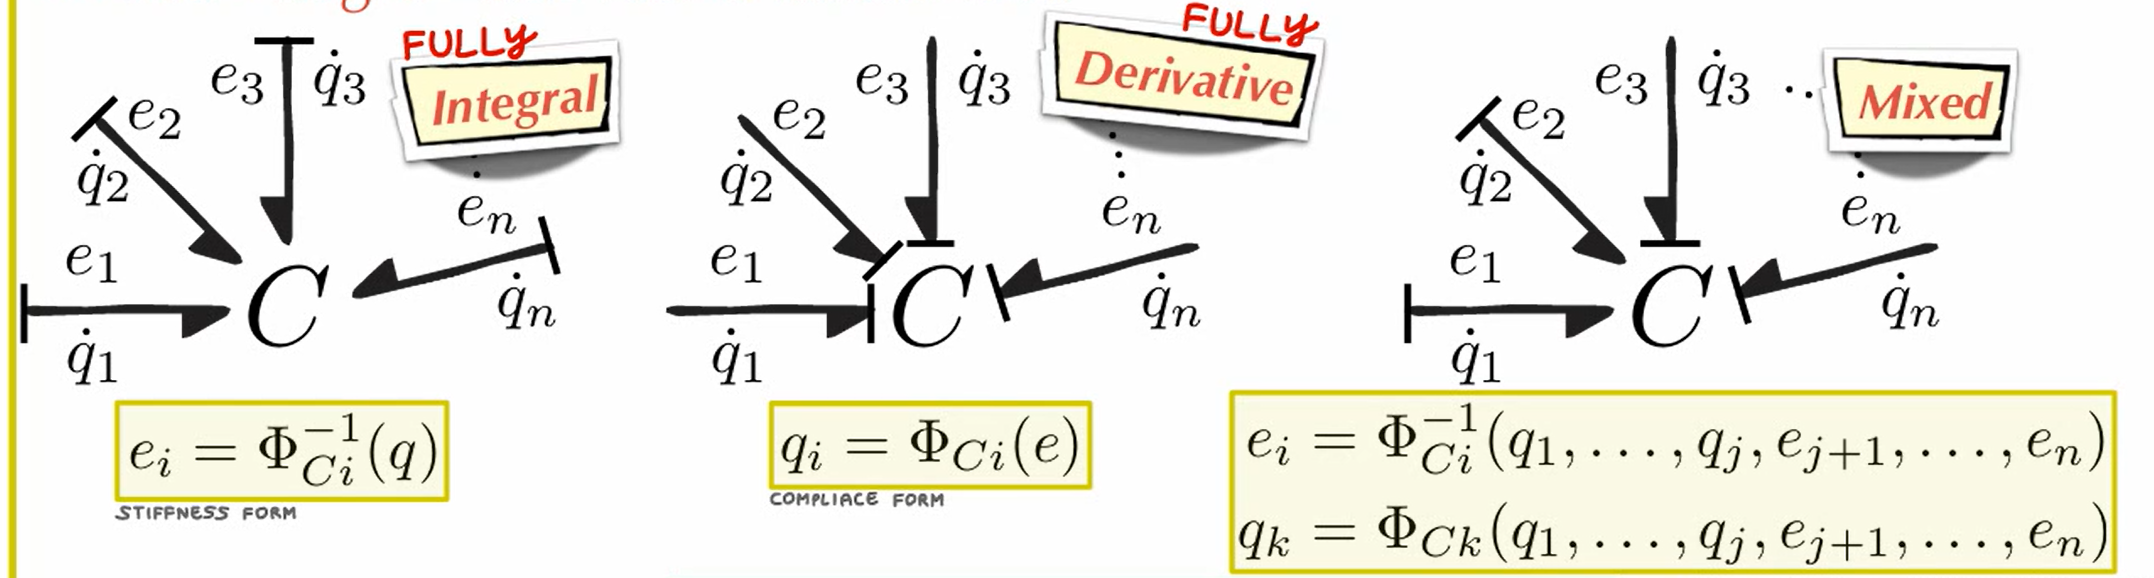
\includegraphics[scale=0.25]{figs/chapter5/5_4.png}
  \caption{Causality in C-fields}
\end{figure}




\begin{insightbox}[Example of causality assignment in a C-field]
  \begin{enumerate}
    \item Draw bond graph
    \item Assign causality
    \item Express the C-field
  \end{enumerate}

  \begin{figure}[H]
    \centering
    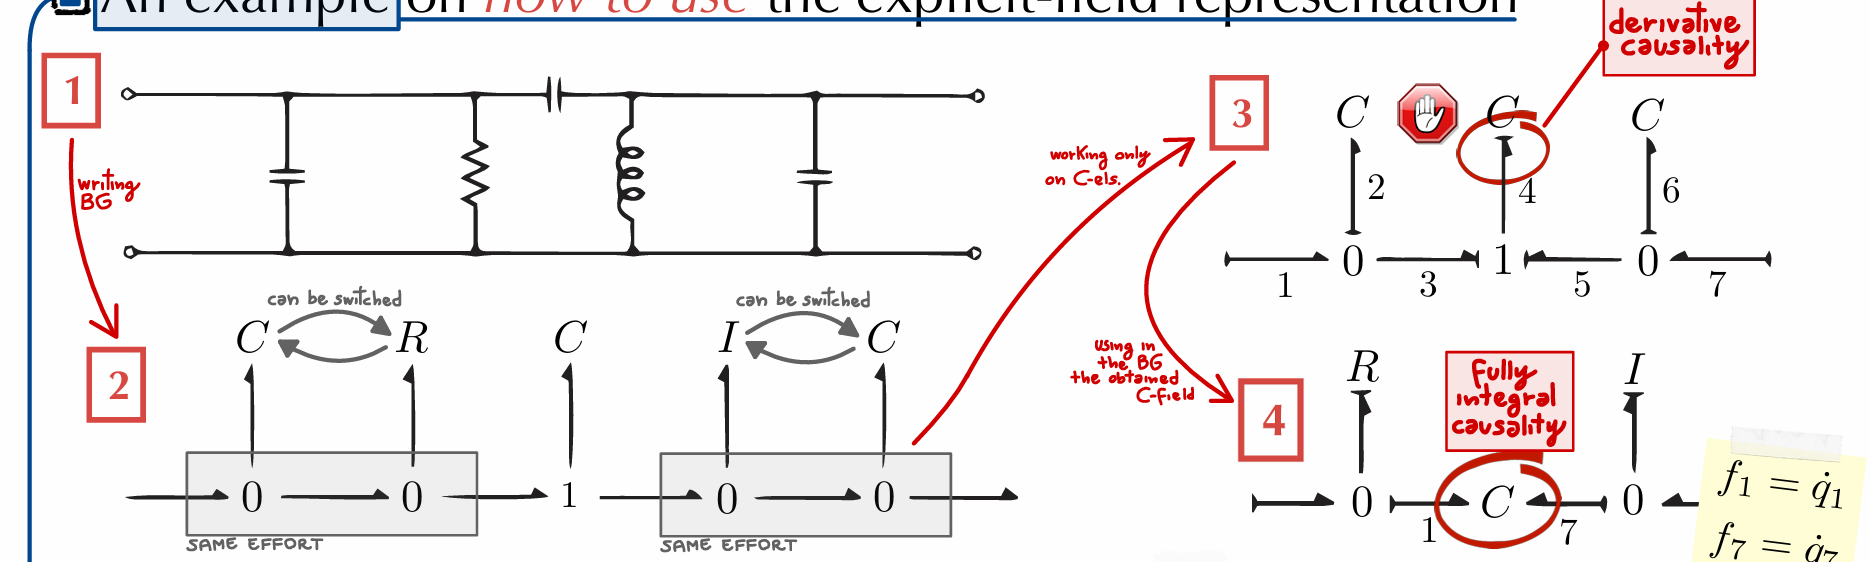
\includegraphics[scale=0.25]{figs/chapter5/5_5.png}
    \caption{Example of causality assignment in a C-field}
  \end{figure}

  The manipulation from implicit to explicit field can be of help if one or more elements must be assigned derivative causality.

  \begin{itemize}
    \item The transformation in an explicit form simplifies equation formulation
    \item This process increases the insight into the \textbf{causes} of derivative causality
    \item The explicit-field representation can be used to avoid the necessity of handling derivative causality. 
  \end{itemize}

  

  It's important to note that when assigning causality, even if an element is assigned in derivative causality, it does not necessarily mean that the resulting constitutive equations will be in derivative form. The derivate causallity of the element is holded inside the C-field, but not externally, at the terminal side. From the terminal point of view, this is just a C-field in fully integral causality. 

  The causality of the inner elements it is not visible from the outside. This is a key point to understand when working with fields.
  
\end{insightbox}


In \textbf{fully integral causality}, all flows are inputs and all efforts are outputs: $\mathbf{e} = \mathbf{K}\,\mathbf{q}$ (stiffness form). In \textbf{fully derivative causality}, all efforts are inputs and all displacements are outputs: $\mathbf{q} = \mathbf{C}\,\mathbf{e}$ (compliance form). \textbf{Mixed causality} involves both, requiring a mixed-form constitutive law obtained by partially inverting the stiffness/compliance matrix. 

For an implicit field, admissible causal forms are easily determined by propagating the standard bond graph causality rules through its constituent elements (e.g., studying conflicts at 0 or 1 junctions). For an explicit field specified in a particular causal form, the question is an algebraic one (whether the constitutive equations can be inverted), and for nonlinear fields, this can be very hard to decide. Notice that, in principle, any strictly valid C-field can always go into fully integral causality!

\section{I-fields: multiport kinetic energy storage}

For I-fields we can develop a complete parallel dual formulation with respect to C-fields. Inertial fields are the exact duals of capacitive fields. The \textbf{I-field} is the multiport generalisation of the 1-port I-element. Its kinetic energy is a function of all momenta simultaneously:

\begin{equation}
  E(\mathbf{p}) = \int_{0}^{t} \sum_{i=1}^{n} e_i f_i d\tau = 
  \int_{0}^{t} \sum_{i=1}^{n} f_i \dot{p}_i d\tau = 
  \int_{0}^{t} \sum_{i=1}^{n} f_i (\mathbf{p}) dp_i =  
  \int_{\mathbf{p}_0}^{\mathbf{p}} \mathbf{f}(\bar{\mathbf{p}})^T\,d\bar{\mathbf{p}}, \qquad
  f_i = \frac{\partial E}{\partial p_i}(\mathbf{p}).
\end{equation}


In the linear case, the energy is $E(\mathbf{p}) = \frac{1}{2}\mathbf{p}^T\mathbf{M}^{-1}\mathbf{p}$. The constitutive law maps momenta to flows via the inverse mass/inertia matrix $\mathbf{M}^{-1}$ (i.e. $\mathbf{f} = \mathbf{M}^{-1}\mathbf{p}$). 

The Maxwell reciprocal relations for I-fields require $\partial f_i/\partial p_j = \partial f_j/\partial p_i$, which translates to the symmetry of $\mathbf{M}^{-1}$ (and hence of $\mathbf{M}$). Like C-fields, I-fields occur in both implicit and explicit forms, and manipulating them can yield highly useful simplified representations.

The most important mechanical physical I-field is the \textbf{3D rigid body}: it has three translational and three rotational momentum ports, with the (constant) mass-inertia tensor providing the constitutive law. In 2D, the I-field reduces to two translational inertias and one rotational inertia, as discussed in Chapter~3. By transforming an implicit rigid-body I-field into an explicit one, we can define the relationship between the center-of-mass velocity and the velocities of the attachment points analytically.


\paragraph{Interacting Coils (Mutual Inductance).}
Another classic use of I-fields is in electrical circuits containing mutually interacting coils. These are conveniently represented using explicit I-fields in derivative causality. To write the constitutive laws, one needs a sign convention for currents/voltages and a convention for the relative orientation of the coils (often denoted by dots, squares, or triangles on schematic diagrams).

If the currents $i_1$ and $i_2$ are defined so that when positive they both enter the dotted ends, the mutual-inductance effects $M$ are positive:
\begin{equation}
  \begin{pmatrix}\lambda_1\\\lambda_2\end{pmatrix} = \begin{pmatrix}L_1 & M_{12}\\ M_{12} & L_2\end{pmatrix}\begin{pmatrix}i_1\\i_2\end{pmatrix}
\end{equation}
If one current enters a dot and the other leaves a dot, the mutual terms become $-M_{12}$. Independently of the coil orientation convention, the inductance matrix and its inverse will always be symmetric as long as the I-field is conservative.

\begin{figure}[H]
  \centering
  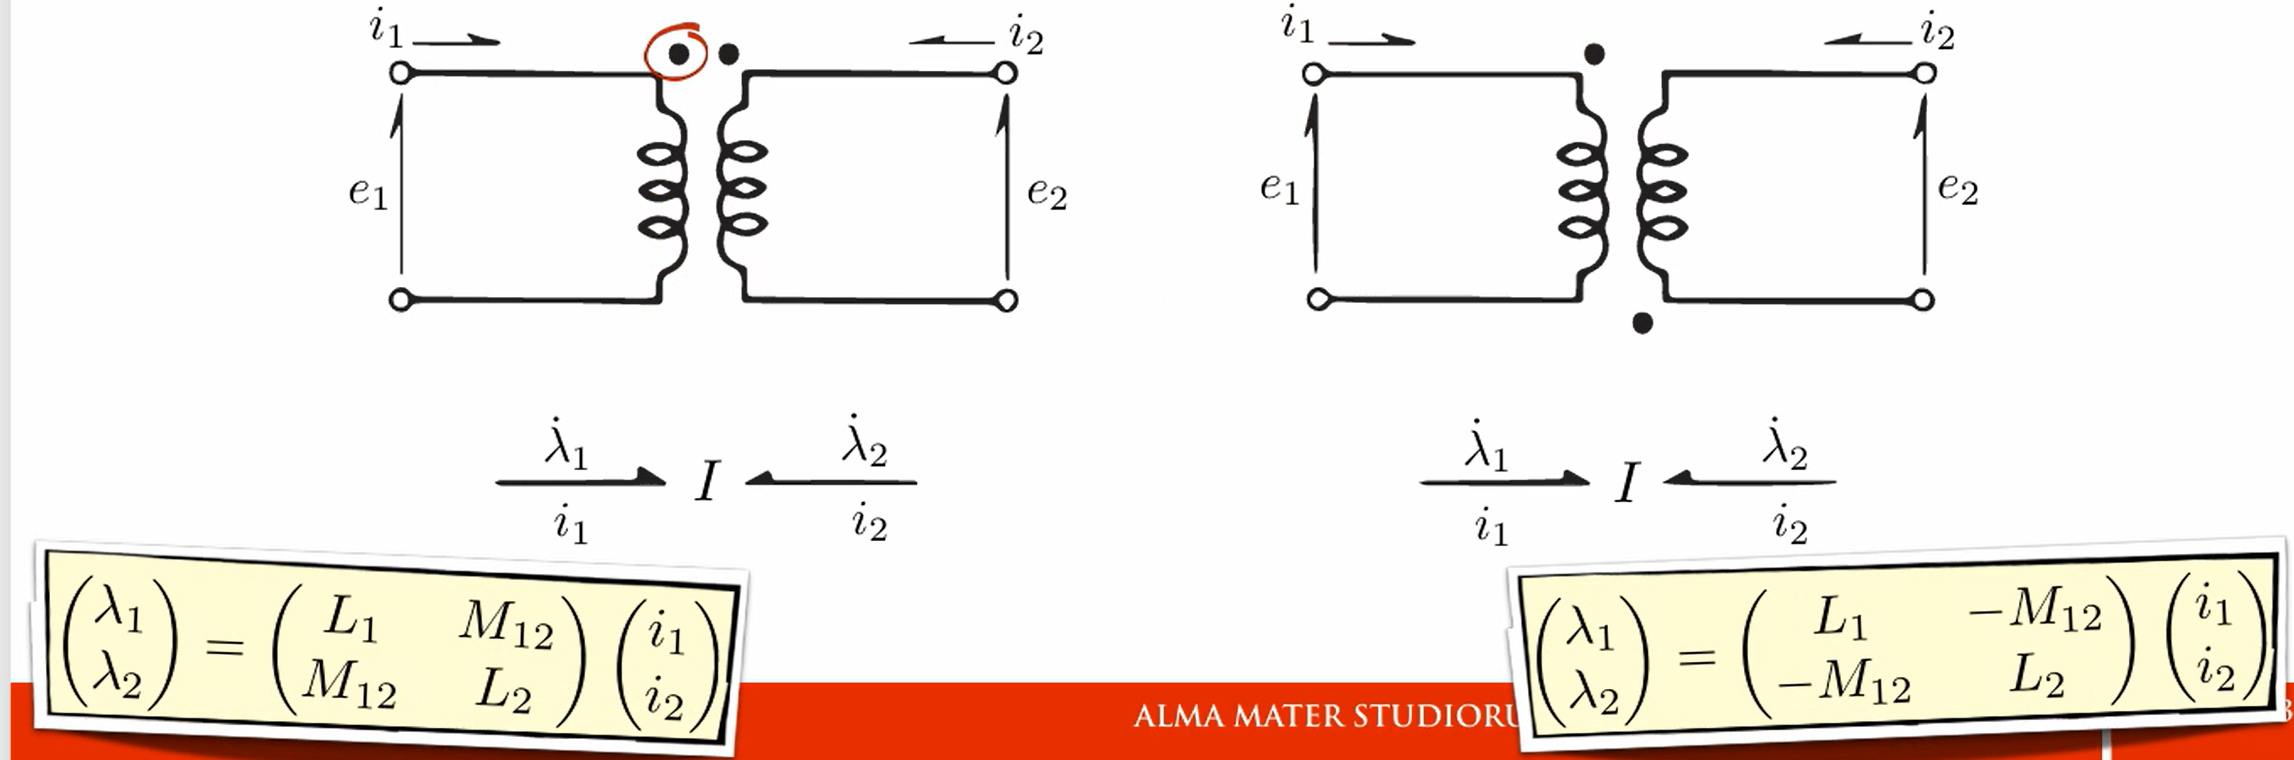
\includegraphics[scale=0.25]{figs/chapter5/5_6.png}
  \caption{Mutually interacting coils represented as an I-field}
\end{figure}


\section{Mixed energy-storing fields (IC-fields)}

There are cases when an energy-storing device acts as a C-field at some ports and an I-field at others. Within a single energy domain, there is usually no need for such an element. However, energy transducers are often ideally energy conservative but store and release energy across different domains over time (e.g., storing electrical energy and releasing it as mechanical work). Because their electrical and mechanical energies are dynamically coupled, they cannot be modeled by simple 1-port C or I elements. You must use a mixed \textbf{IC-field} to mathematically capture the complex physics natively.


For an IC-field with momentum variables $p$ and displacement variables $q$, the total energy features dynamic coupling (an irrotational case) and contains mixed terms. The constitutive equations are obtained by taking the appropriate partial derivatives of the total stored energy $E(p, q)$. 

\begin{equation}
  E(\mathbf{p}) = \int_{0}^{t} \sum_{i=1}^{n} e_i f_i d\tau = 
  \int_{0}^{t} \sum_{i=1}^{j} f_i \dot{p}_i d\tau + \int_{0}^{t} \sum_{k=j+1}^{n} e_k \dot{q}_k d\tau
\end{equation}

Maxwell's reciprocal relations for IC-fields require that the mixed second derivatives of the energy function are equal:
\begin{equation}
  \frac{\partial^2 E}{\partial p_i \partial q_k} = \frac{\partial^2 E}{\partial q_k \partial p_i} \quad \forall\, i, k.
\end{equation}


\begin{figure}[H]
  \centering
  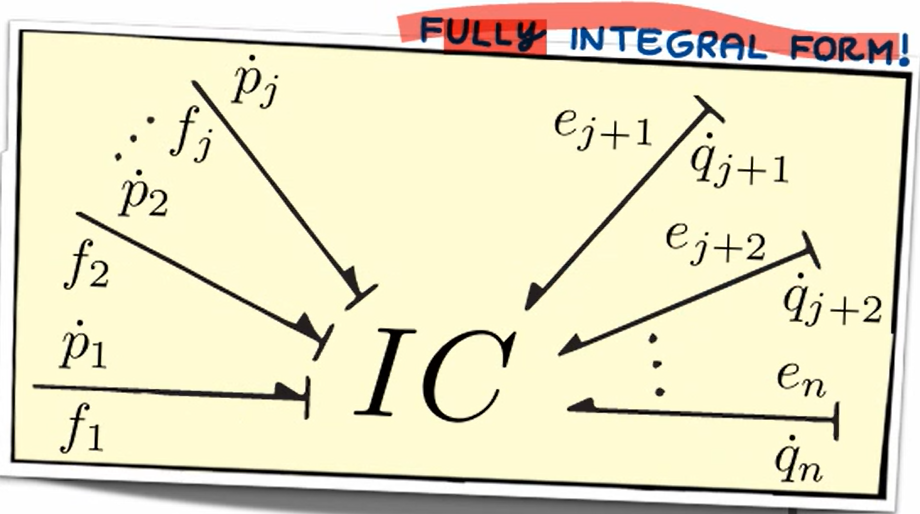
\includegraphics[scale=0.25]{figs/chapter5/5_7.png}
  \caption{IC-field with two I-ports and two C-ports}
\end{figure}

\begin{example}[Movable-Plate Capacitor]
A capacitor where one plate can move mechanically acts as a C-port electrically (charge $q$) and a C-port mechanically (position $x$). The stored energy is $E(q,x) = \frac{1}{2}\frac{q^2}{C(x)}$. The constitutive equations are:
\begin{equation}
    e = \frac{\partial E}{\partial q} = \frac{q}{C(x)} \qquad \text{and} \qquad F = \frac{\partial E}{\partial x} = -\frac{1}{2}\frac{q^2}{C^2(x)}\frac{\partial C}{\partial x}
\end{equation}

\begin{figure}[H]
  \centering
  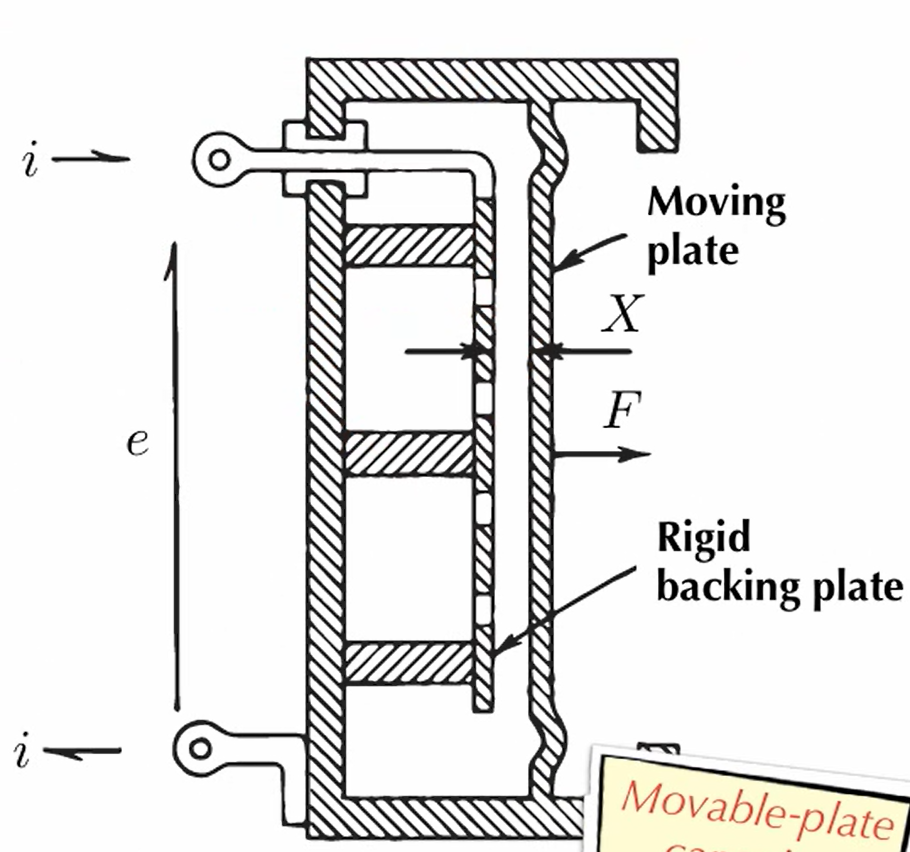
\includegraphics[scale=0.25]{figs/chapter5/5_8.png}
  \caption{Movable-plate capacitor as an IC-field}
\end{figure}

\end{example}




\begin{example}[Electrical Solenoid]
The electrical solenoid serves as a prototype of an IC-field transducer. From the electrical port, the coil exhibits self-inductance ($\lambda$). From the mechanical port, the force on the slug depends on its position ($x$). The energy is $E(\lambda,x) = \frac{1}{2}\frac{\lambda^2}{L(x)}$. The constitutive equations are:
\begin{equation}
    i = \frac{\partial E}{\partial \lambda} = \frac{\lambda}{L(x)} \qquad \text{and} \qquad F = \frac{\partial E}{\partial x} = -\frac{1}{2}\frac{\lambda^2}{L^2(x)}\frac{\partial L}{\partial x}
\end{equation}

\begin{figure}[H]
  \centering
  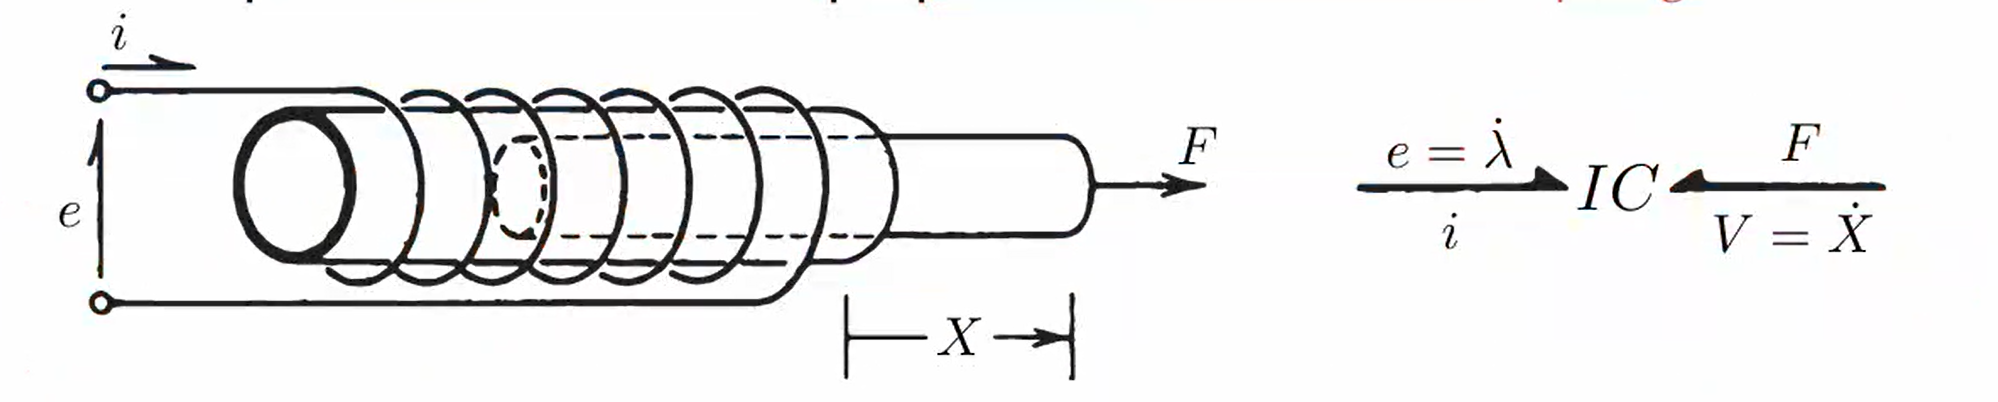
\includegraphics[scale=0.25]{figs/chapter5/5_9.png}
  \caption{Electrical solenoid as an IC-field}
\end{figure}

\end{example}


\section{R-fields: multiport dissipation}

An \textbf{R-field} is an $n$-port with a static (or algebraic) constitutive law that relates efforts and flows. In general, R-fields are \textbf{NOT} strictly related or associated to power losses: their TRUE intrinsic characteristic is to algebraically relate efforts and flows! 

This broad definition includes power-conserving elements, such as 0- and 1-junctions, and elements containing sources. However, in practice, most explicit R-fields do dissipate power (e.g. thermal resistors, coupled fluid friction matrices). Explicit R-fields arise frequently in modelling nonlinear devices.

The causality of an R-field is determined by the sources and energy-storing elements attached to it. 
\begin{itemize}
    \item \textbf{Resistance causality:} All flows are inputs, efforts are outputs ($e_i = \Phi_{R_i}(f_1 \dots f_n)$).
    \item \textbf{Conductance causality:} All efforts are inputs, flows are outputs ($f_i = \Phi_{R_i}^{-1}(e_1 \dots e_n)$).
    \item \textbf{Mixed causality:} A mixture of effort and flow inputs. 
\end{itemize}


\begin{figure}[H]
  \centering
  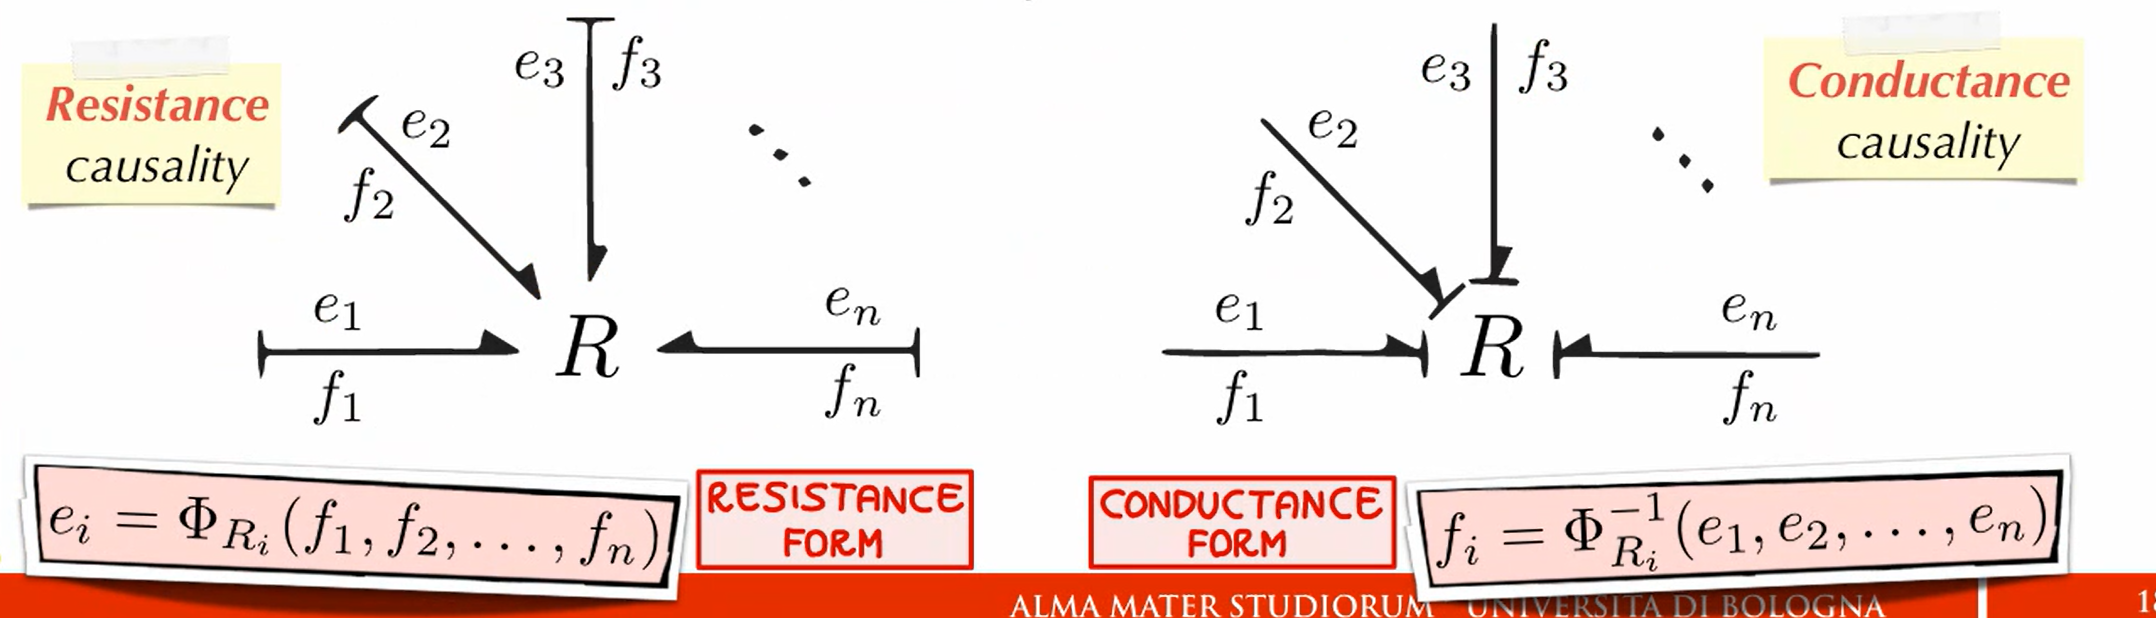
\includegraphics[scale=0.25]{figs/chapter5/5_10.png}
  \caption{Causality in R-fields}
\end{figure}

\paragraph{Onsager vs. Casimir Forms and Power.}
Since an R-field has no stored energy function, there is no direct equivalent to Maxwell's Reciprocal Relations. However, structural properties do exist. Any square Constitutive Law Matrix (CLM) $M$ can always be mathematically decomposed into a symmetric part $M_S = \frac{1}{2}(M+M^T)$ and a skew-symmetric (antisymmetric) part $M_A = \frac{1}{2}(M-M^T)$. 

The asymmetric contribution $M_A$ is always related to \emph{perfectly conserved power} ($P_w = b^T M_A b = 0$). The symmetric part $M_S$ is associated with power dissipation.

Implicit R-fields composed strictly of linear 1-port resistances, 0-junctions, 1-junctions, and transformers will obey \textbf{Onsager Reciprocity}: when expressed in pure resistance or conductance form, their CLM is perfectly symmetric (called the \emph{Onsager form}). When expressed in mixed causality, the matrix is guaranteed to present asymmetric terms. 

Importantly, NOT all R-fields obey Onsager Reciprocity. If Gyrators (GY) are allowed inside the implicit R-field, the reciprocity is broken, yielding asymmetric terms even in pure resistance/conductance forms. This is known as the \textbf{Casimir form}.

There could be examples of R-fields that are not Onsager and Casimir at the same time, but a mix of the two. 

\begin{figure} [H]
  \centering
  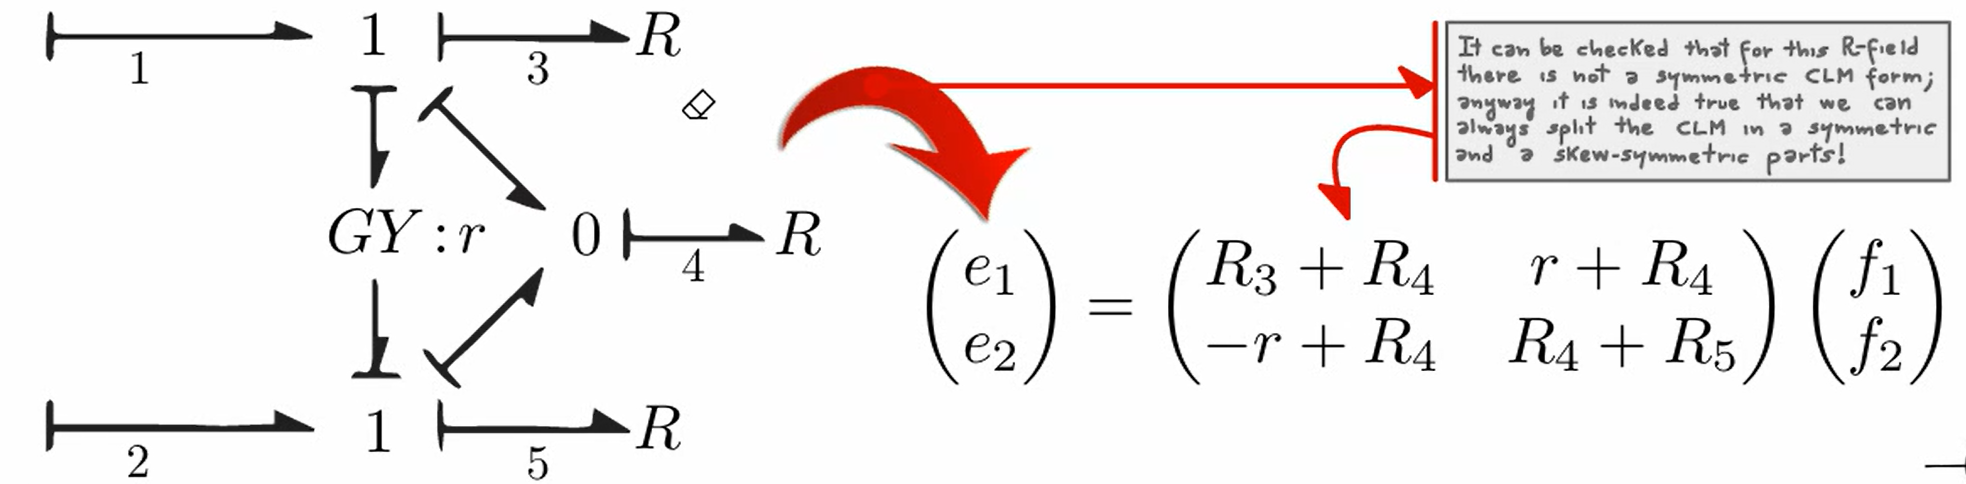
\includegraphics[scale=0.25]{figs/chapter5/5_11.png}
  \caption{R-field without Onsager and Casimir reciprocity}
\end{figure}


\section{Modulated 2-port elements}

Before discussing pure junction structures, it is essential to introduce the modulated 2-ports. The \textbf{modulated transformer (MTF)} and \textbf{modulated gyrator (MGY)} are nonlinear, power-conserving generalisations of TF and GY. 

The parameters (modulus $m$ or $r$) of these elements are allowed to be a function of some other parameter in the system (often a displacement or angle, possibly time-varying). These parameters are modulated by means of a signal (active bond) rather than a power bond. Thus, it is characteristic of these elements that the parameters change value without a directly associated power flow!

Examples include the DC motor (Faraday \& Lorentz laws modelled as an MGY depending on field current) and the slider-crank or rack-and-pinion mechanisms (modelled as MTF). 


\section{Junction structures}

\textbf{Junction structures} are the energy switchyards that enforce the constraints among parts of dynamic systems. They result from the interconnection of 0-junctions, 1-junctions, TF, and GY. They contain no dissipative or storage elements.

Junction structures are essentially special types of R-fields that \emph{never} dissipate power (meaning their CLM is completely skew-symmetric). They are always \textbf{anti-symmetric} because they cannot dissipate power. Because they cannot dissipate power, they typically \textbf{cannot} accept all possible causal assignments at their ports (e.g., a pure junction structure without gyrators cannot accept resistance or conductance causality on all ports simultaneously).

Junction structures have a key property: they are themselves power-conserving, so $\sum_k e_k f_k = 0$ across all their external ports. Equivalently, the junction structure defines a set of linear constraints (from the junctions) and scaling/exchange rules (from TF and GY) on the port variables.

\begin{figure}[H]
  \centering
  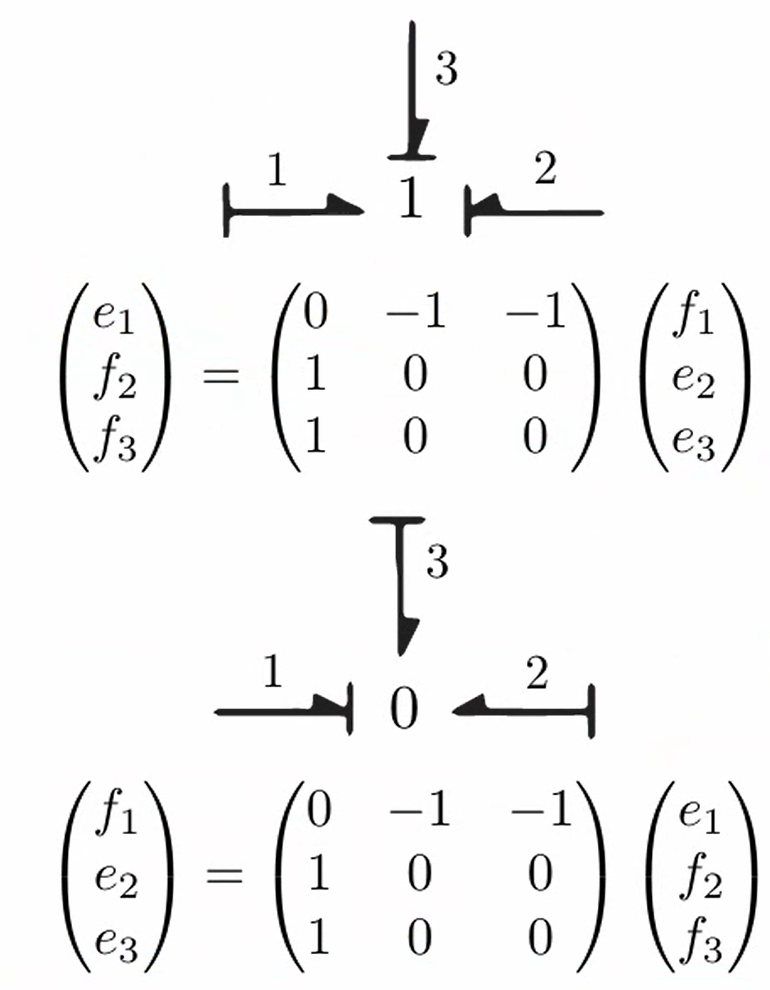
\includegraphics[scale=0.25]{figs/chapter5/5_12.png}
  \caption{Junction structure as a power-conserving R-field}
\end{figure}


\subsection{Multiport Transformers (Kinematics)}

Another extremely interesting viewpoint about junction structures involves the transformations of variables they provide. A \textbf{multiport transformer} is a specific assemblage of 0s, 1s, and TFs that shows more than two ports to the external world. 

Mathematically, a multiport transformer is characterised by a matrix $\mathbf{G}$ and its transpose $\mathbf{G}^T$, just as a 2-port transformer is characterised by a single modulus $m$. By setting a "through" power convention (power in for inputs, out for outputs), the constitutive law can always be written as:

\begin{equation}
    \mathbf{e}_{in} = \mathbf{G} \cdot \mathbf{e}_{out} \qquad \text{and} \qquad \mathbf{f}_{out} = \mathbf{G}^T \cdot \mathbf{f}_{in}
\end{equation}

\begin{figure}[H]
  \centering
  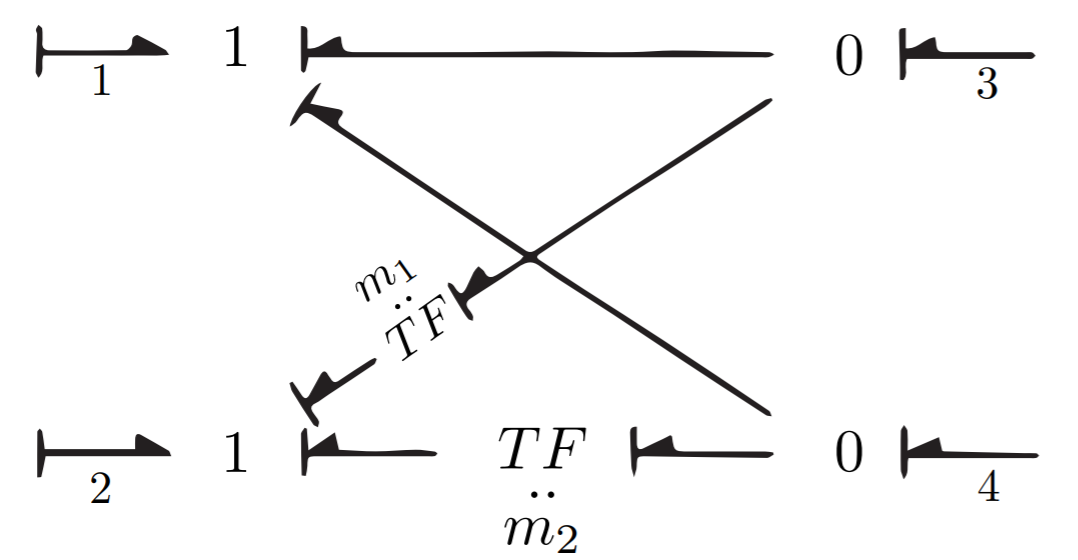
\includegraphics[scale=0.25]{figs/chapter5/5_13.png}
  \caption{Multiport transformer as a power-conserving R-field}
\end{figure}


This is exactly the formulation used for 3D Kinematics and coordinate transformations! A typical example is implementing a Jacobian $J(q)$ that links a joint-coordinate space to a Cartesian-coordinate space in robotics. The forward kinematics ($\dot{x} = J(q)\dot{q}$) dictates the flow transformations, and by power conservation, the transpose Jacobian dictates the force-torque effort transformations ($T = J^T(q)F$). Grouping these into a multiport MTF field elegantly handles 3D kinematics directly within the bond graph framework.

